% Définition du répertoire contenant les images
\graphicspath{{IMAGE/}}

% FRAME Intro
\begin{frame}


\includegraphics[width=12cm]{Logos.pdf}

\vfill

\begin{center}

\vspace*{1.5cm}

\LARGE
\textbf{Sémiologie graphique et travail de l'image}

\vspace*{2.5cm}

\large

\textbf{Hadrien Commenges}

{\small

\vspace*{0.1cm}

\url{hadrien.commenges@univ-paris1.fr}}

\end{center}

\end{frame}

% FRAME
\begin{frame}{Inventaire des situations cartographiques}

\begin{figure}
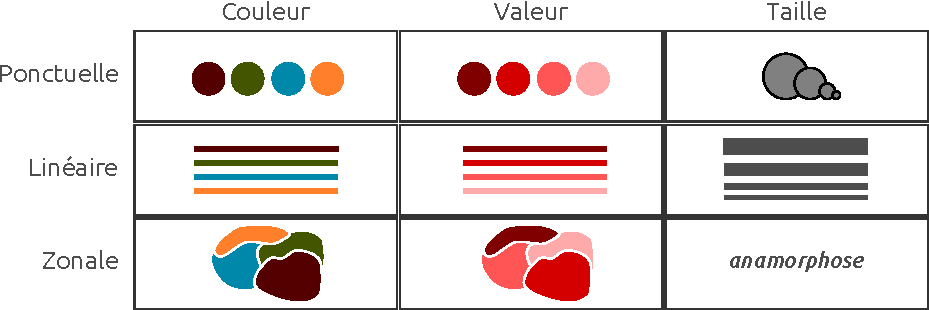
\includegraphics[width=12cm]{semio1.pdf}
\end{figure}

\end{frame}

% FRAME
\begin{frame}{Inventaire des situations cartographiques}

\begin{figure}
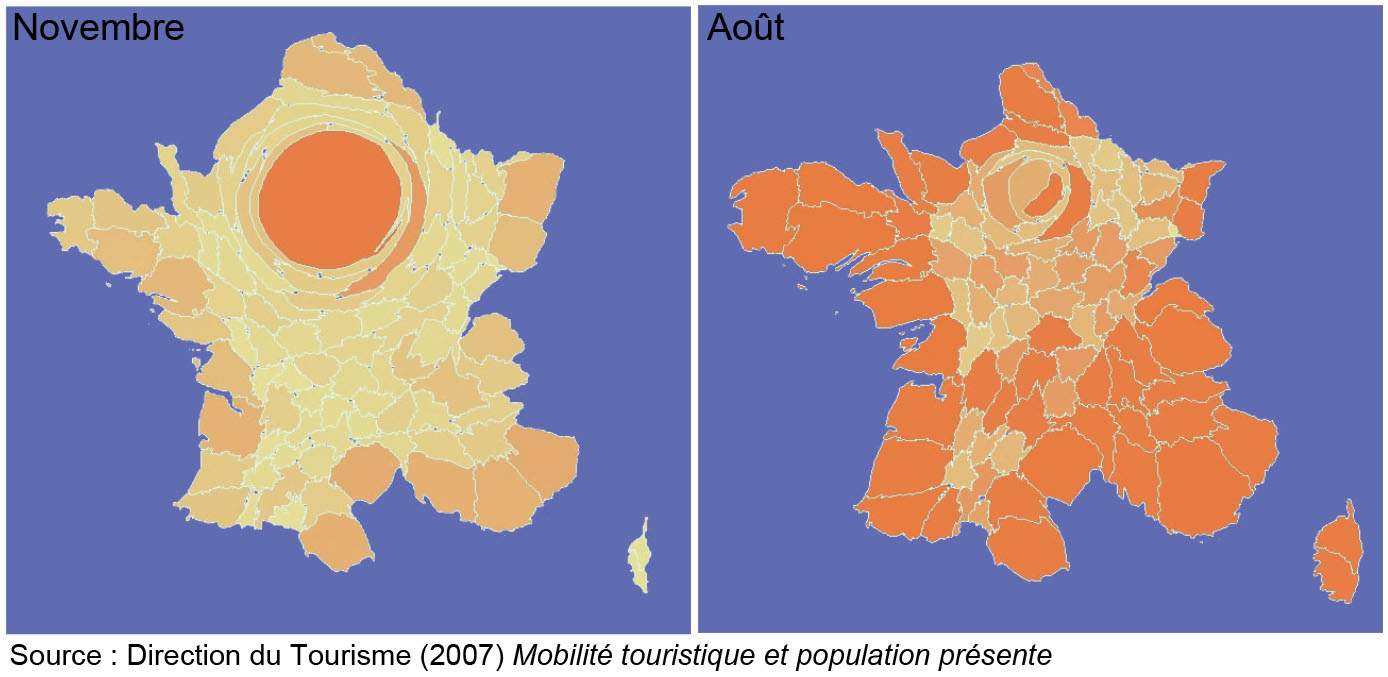
\includegraphics[width=12cm]{Anamorphose.jpg}
\end{figure}

\end{frame}


% FRAME
\begin{frame}{Inventaire des situations cartographiques}

\begin{figure}
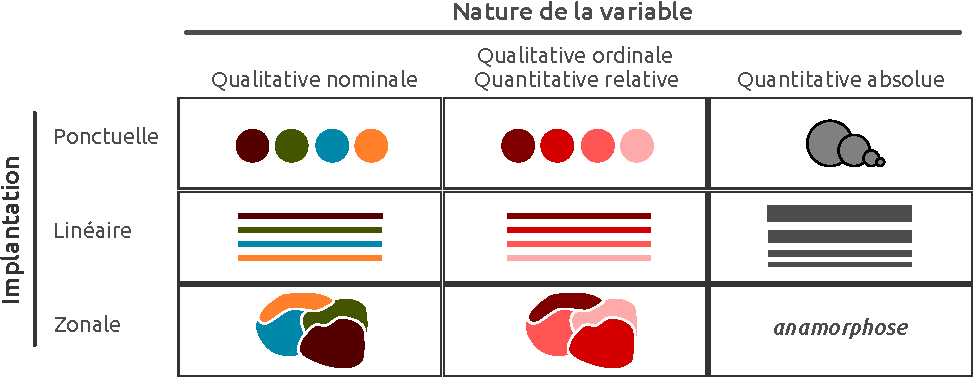
\includegraphics[width=12cm]{semio2.pdf}
\end{figure}

\end{frame}


% FRAME
\begin{frame}{Discrétisation}

\begin{figure}
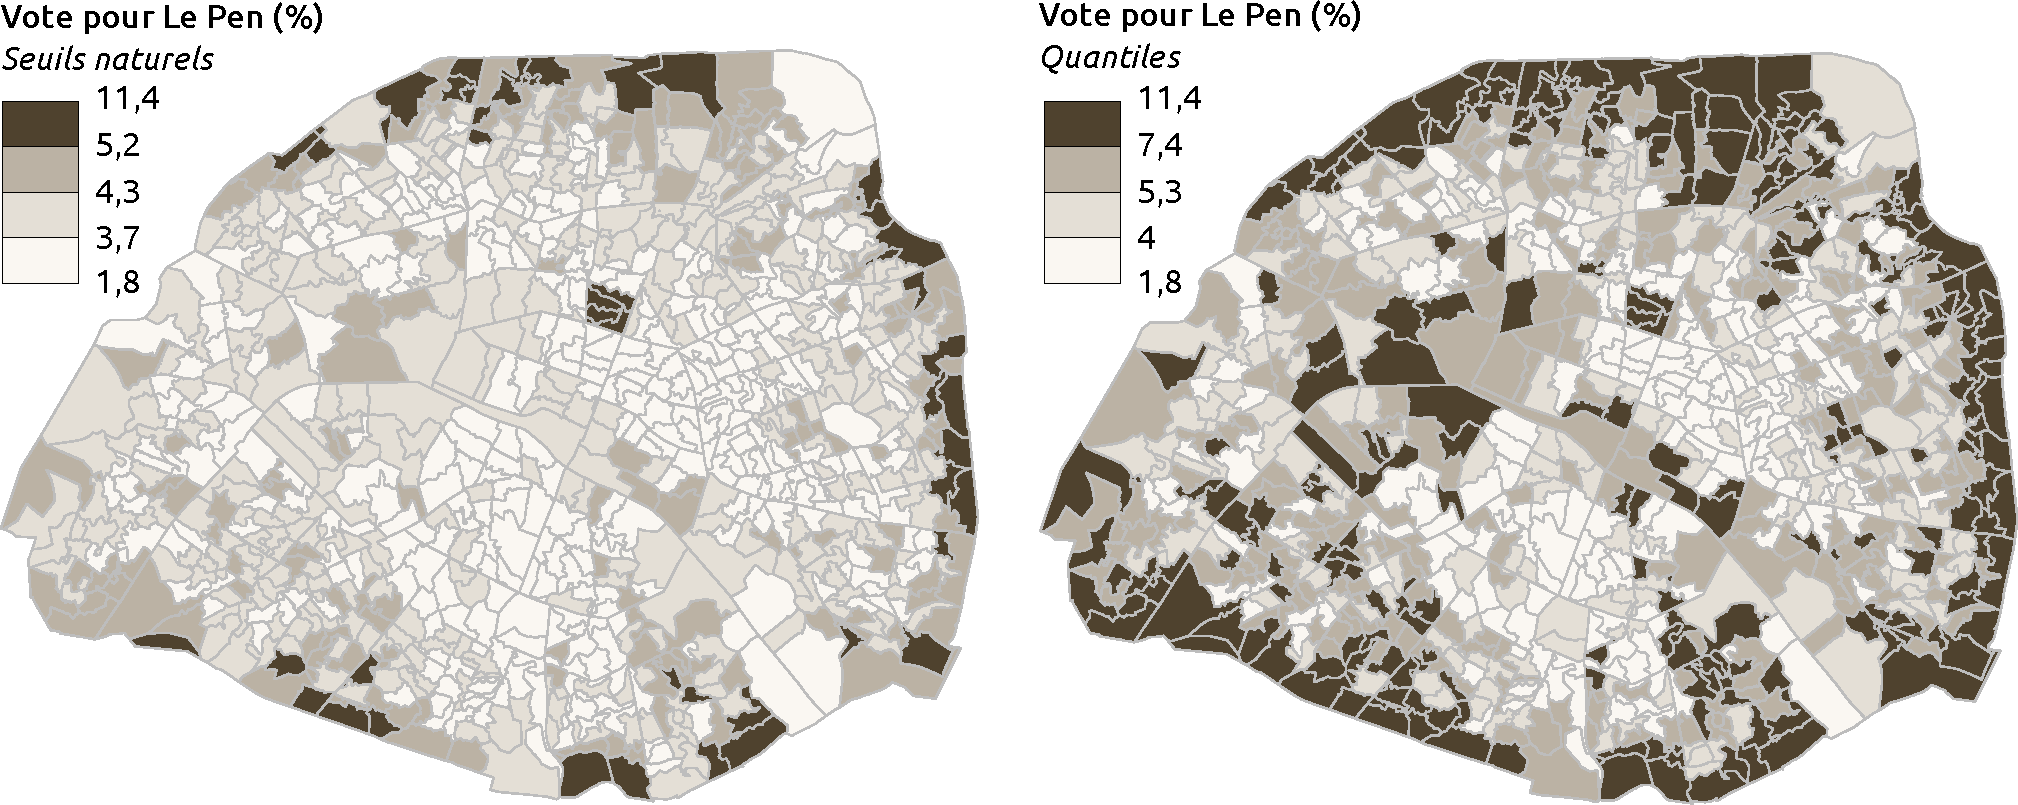
\includegraphics[width=12cm]{Discretisation.pdf}
\end{figure}

~

\textbf{Tester sur ExploratR:} \url{http://shiny.parisgeo.cnrs.fr/ExploratR}

\end{frame}


% FRAME
\begin{frame}{Discrétisation}

\begin{block}{Objectif de la discrétisation}
  Discrétiser c'est rendre discrète une variable continue, i.e. faire des classes: \\
  \textbf{variable quantitative} $\rightarrow$ \textbf{variable qualitative ordinale} \\
  La discrétisation doit rendre compte de la forme de la distribution.
\end{block}


\begin{itemize}
  \item \textbf{Seuils naturels}: fait apparaître des groupes naturels. \\ 
  Ne jamais utiliser pour la comparaison de plusieurs variables.
  \item \textbf{Moyenne et écart-type}: si la distribution est symétrique. \\
  Peut servir à la comparaison si toutes les variables sont symétriques.
  \item \textbf{Amplitudes égales}: peu importe la forme de la distribution. \\
  Peut servir à la comparaison de plusieurs variables.
  \item \textbf{Effectifs égaux}: si la distribution est asymétrique. \\
  Peut servir à la comparaison de plusieurs variables.
\end{itemize}

\end{frame}


% FRAME
\begin{frame}{Habillage}

\begin{figure}
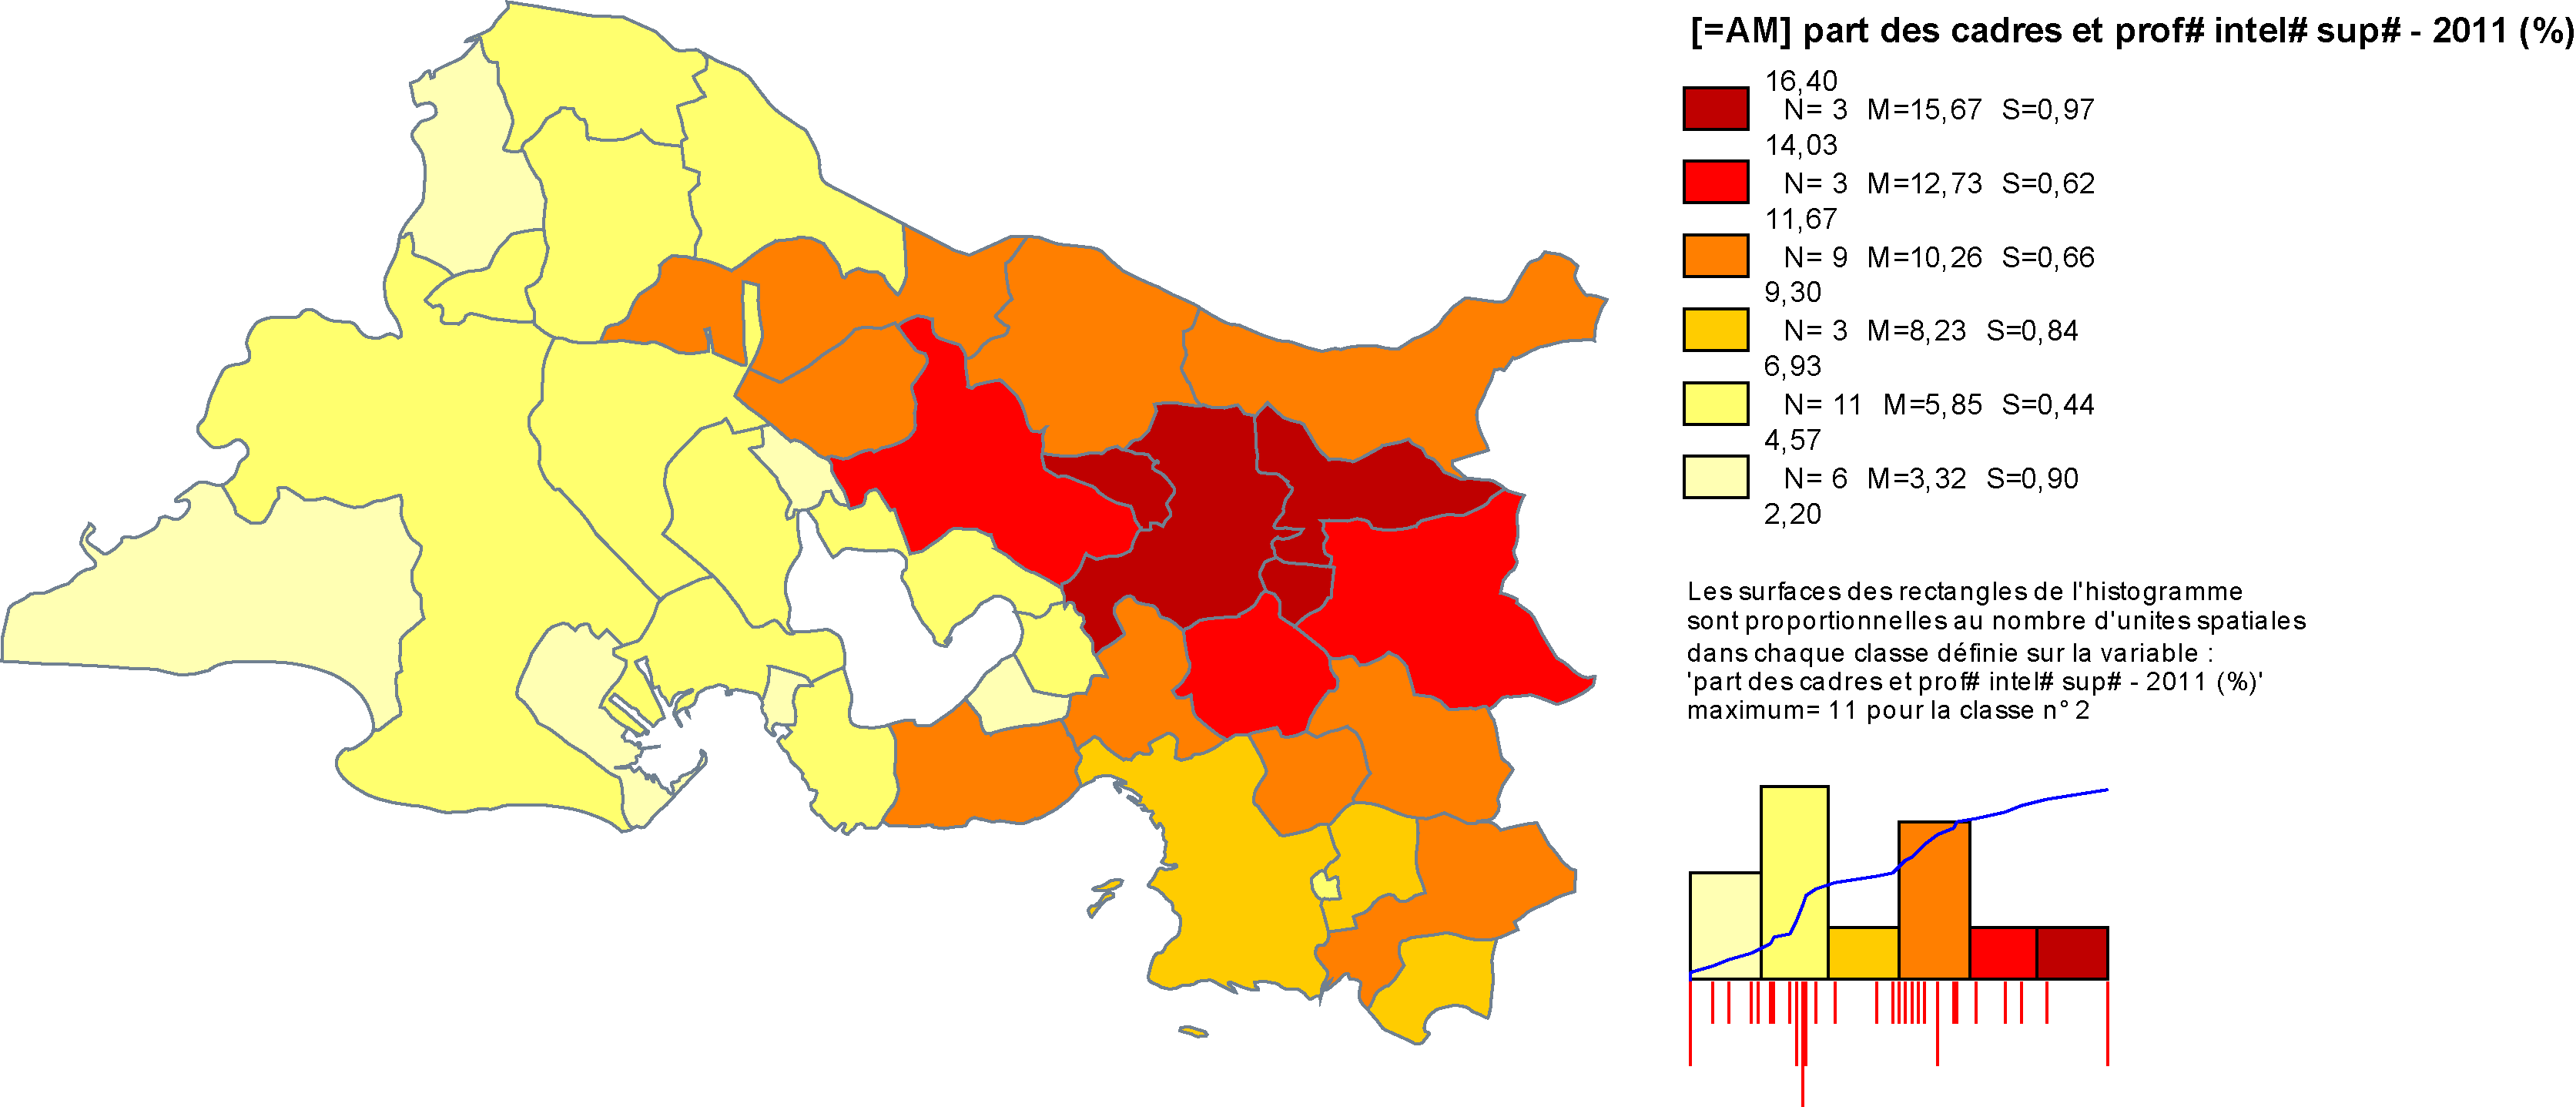
\includegraphics[width=12cm]{CarteCadres.png}
\end{figure}

\end{frame}

% FRAME
\begin{frame}{Habillage}

\begin{block}{Qu'est-ce que l'habillage}
  Ensemble des indications et des figures extérieures à la surface cartographiée (Comité français de cartographie).
\end{block}

Une carte doit être accompagnée a minima des éléments suivants:
\begin{itemize}
  \item \textbf{Titre}: thème, univers et maille. \\ 
  \textit{Évolution de l'agriculture biologique dans les départements français}
  \item \textbf{Titre de légende}: indicateur et unité de mesure. \\
  \textit{Part de la SAU en agriculture biologique (\%)}
  \item \textbf{Légende}: description précise de la variation visuelle. \\
  \textit{Seuils de classe (lisible), discrétisation, catégories}
  \item \textbf{Source} \& \textbf{Auteur}
  \item \textbf{Échelle} \& \textbf{Orientation} (optionnel)
\end{itemize}

\end{frame}


% FRAME
\begin{frame}{Inventaire des situations graphiques}

\textbf{Graphiques univariés}

\begin{figure}
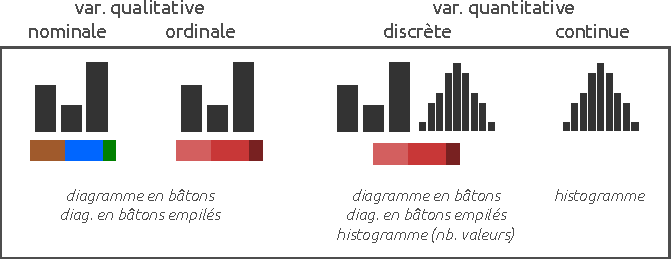
\includegraphics[width=11.5cm]{TableauGraphique.pdf}
\end{figure}

\end{frame}


% FRAME
\begin{frame}{Inventaire des situations graphiques}

\textbf{Graphiques bivariés}

\begin{figure}
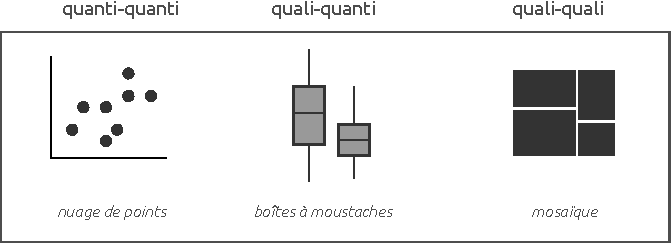
\includegraphics[width=11.5cm]{TableauGraphique2.pdf}
\end{figure}

\end{frame}


% FRAME
\begin{frame}{Boîte à moustaches (\textit{boxplot})}


\begin{figure}
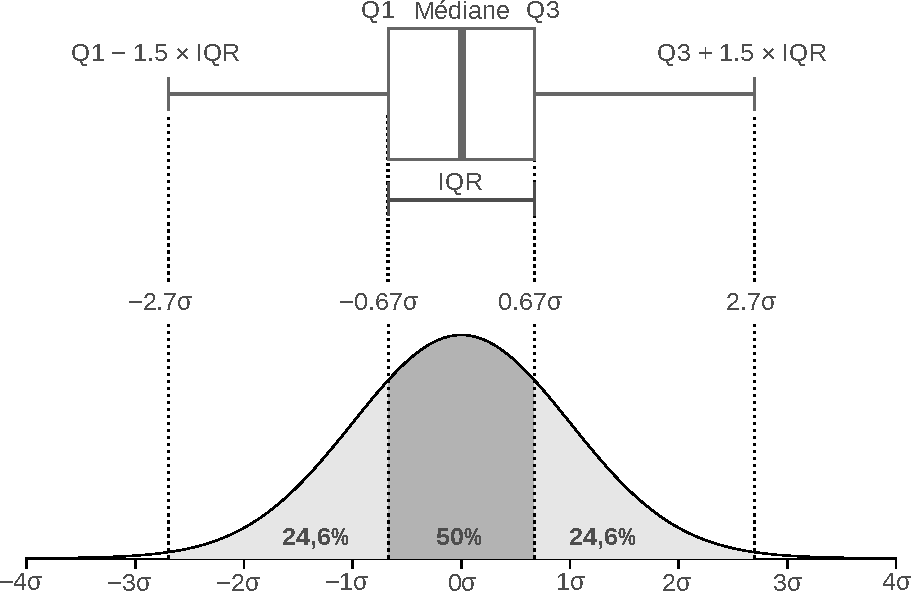
\includegraphics[width=10.5cm]{Boxplot.pdf}
\end{figure}

\end{frame}


% FRAME
\begin{frame}{Mosaïque (\textit{mosaic plot})}

\begin{figure}
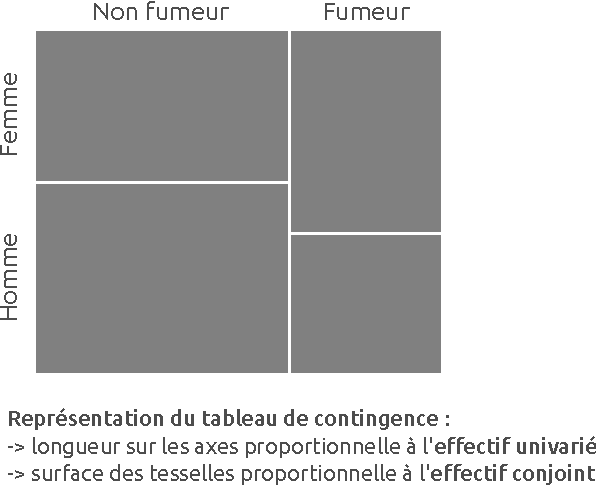
\includegraphics[width=9cm]{Mosaique.pdf}
\end{figure}

\end{frame}


% FRAME
\begin{frame}{Habillage}

Comme les documents cartographiques, \textbf{les graphiques doivent être habillés}:

\begin{itemize}
  \item \textbf{Titre}: thème, univers et maille. \\ 
  \item \textbf{Titre des axes}: indicateur et unité de mesure. \\
  \item \textbf{Légende}: description précise des variations visuelles. \\
  \item \textbf{Source} \& \textbf{Auteur}
\end{itemize}

\end{frame}


% FRAME
\begin{frame}{Travail des images}

La qualité et le poids d'un fichier raster dépendent essentiellement de deux aspects: la \textbf{résolution} (nombre de pixels) et la \textbf{profondeur chromatique} (bits par pixel).

\begin{figure}
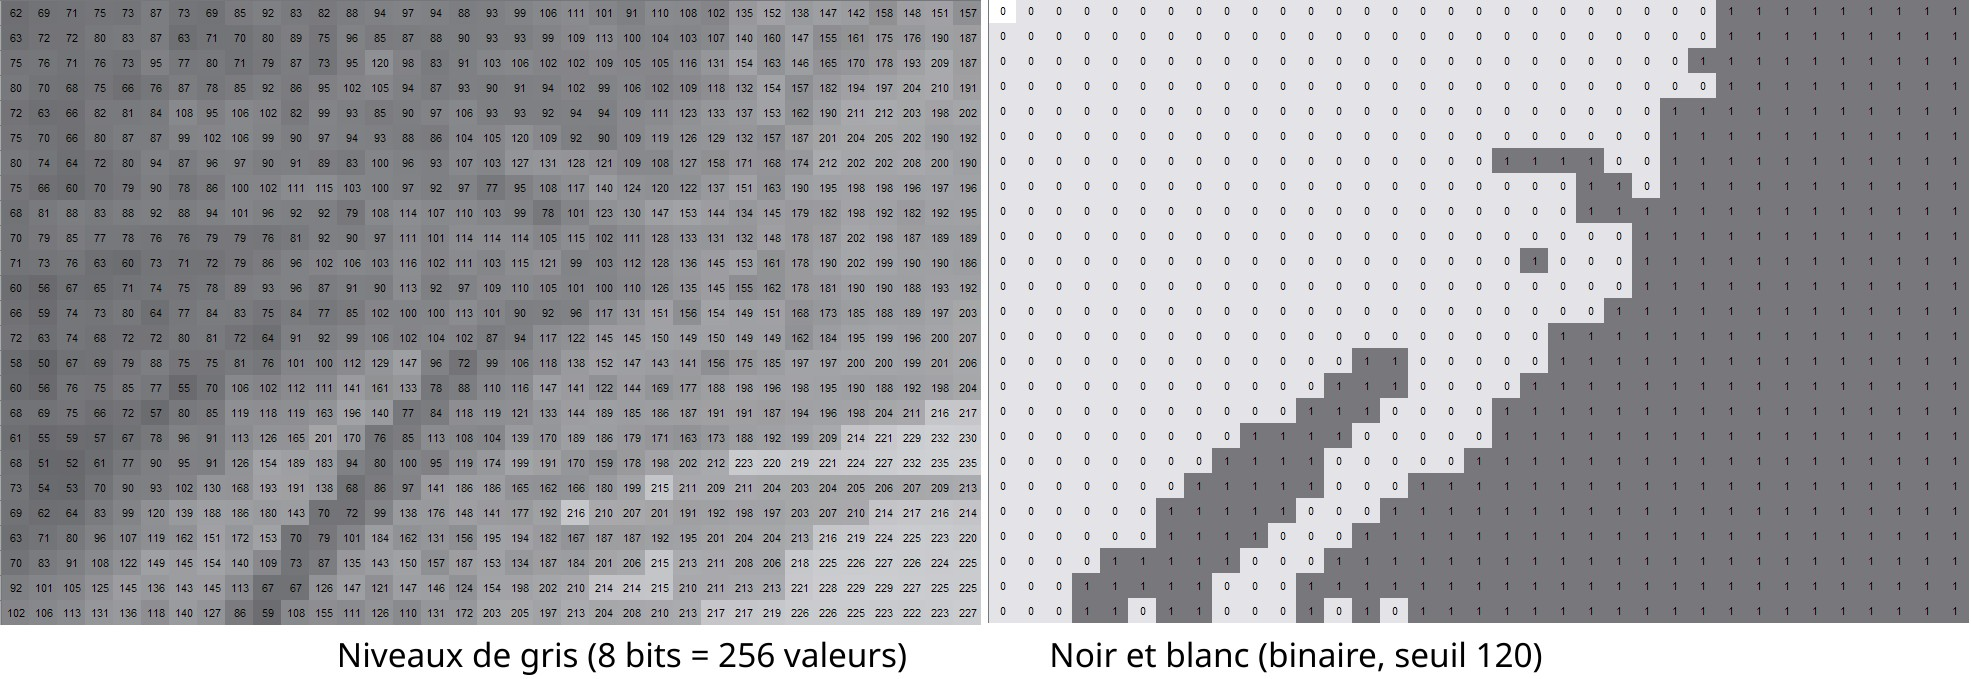
\includegraphics[width=12cm]{EinsteinZoom.jpg}
\end{figure}

\end{frame}


% FRAME
\begin{frame}{Travail des images}

\begin{figure}
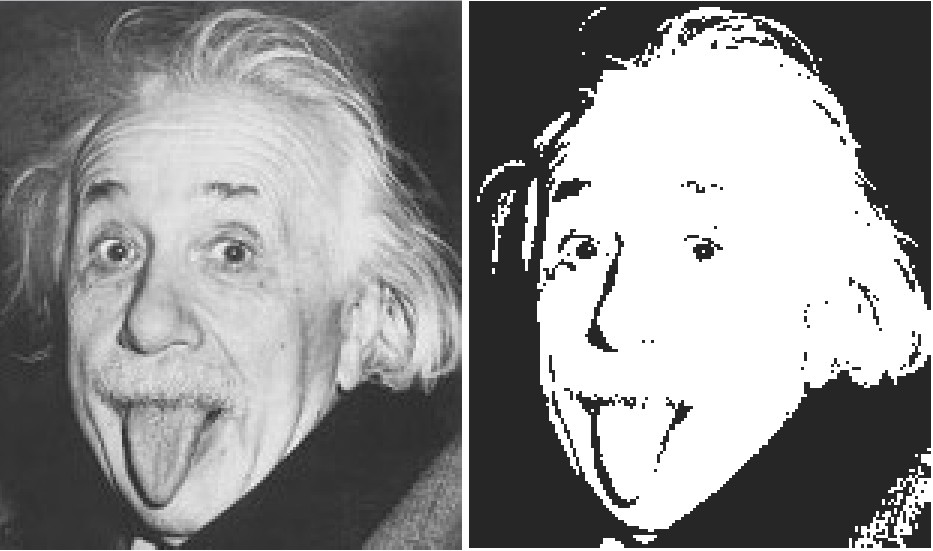
\includegraphics[width=12cm]{Einstein.jpg}
\end{figure}

\end{frame}


% FRAME
\begin{frame}{Travail des images}

\begin{figure}
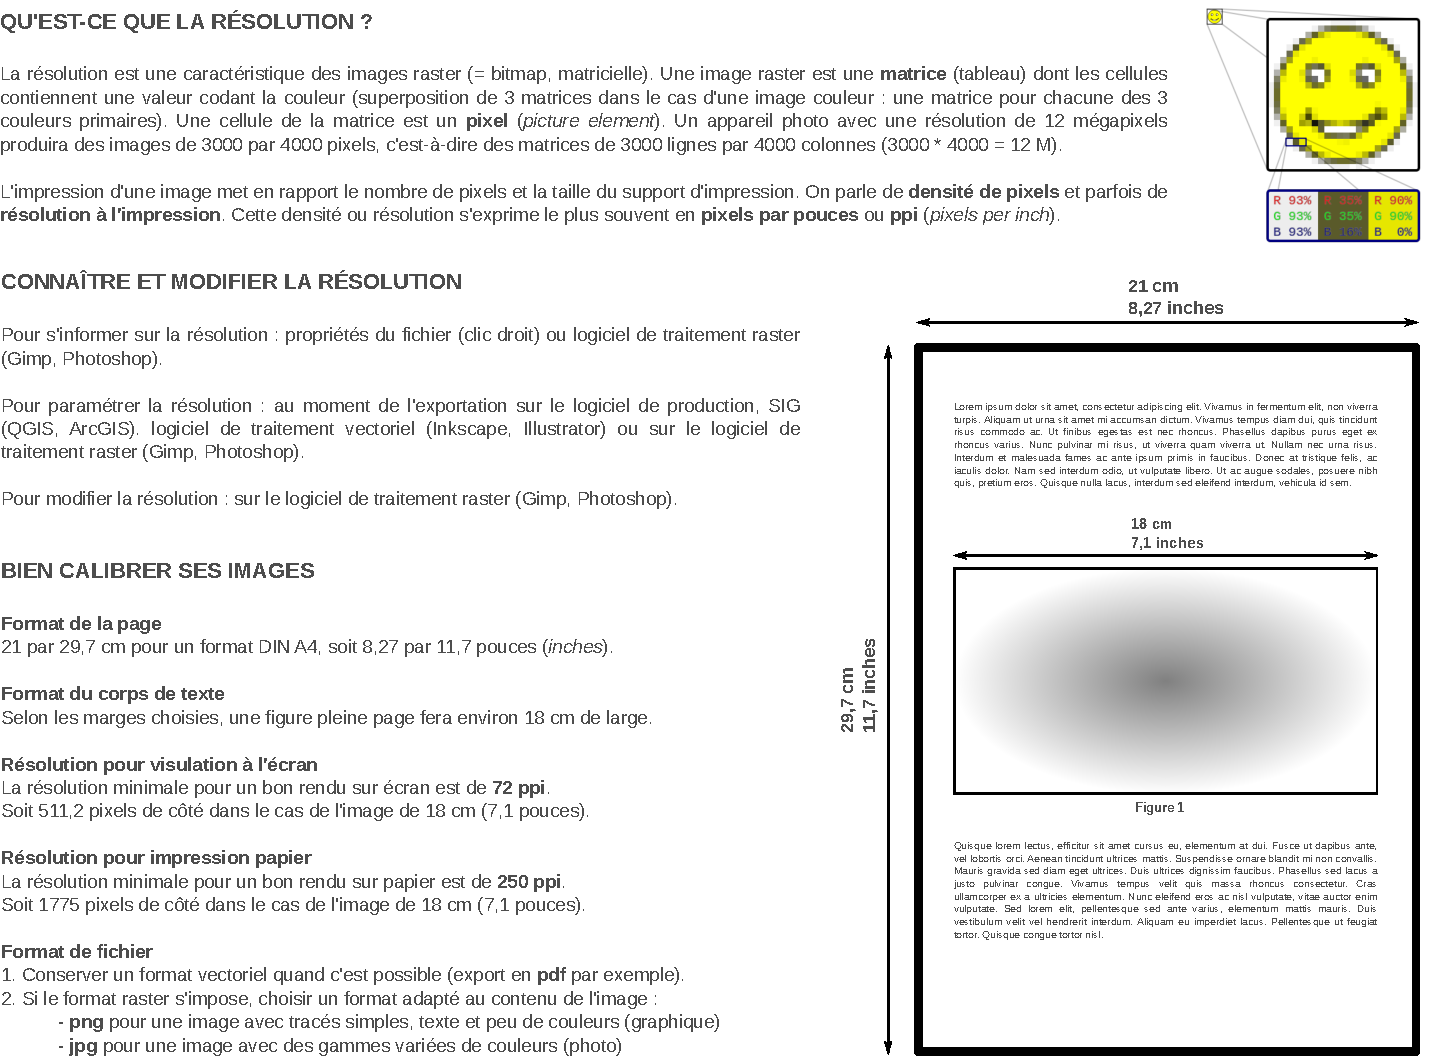
\includegraphics[width=11cm]{ResolutionImages.pdf}
\end{figure}

\end{frame}